\documentclass{article}
\usepackage[utf8]{inputenc}

\usepackage{float}
\usepackage{caption}


\RequirePackage{tabularx}   % Tabulars with adjustable-width columns


\usepackage[table]{xcolor} 
\definecolor{myblue}{HTML}{CCF4FF}
\definecolor{myorange}{HTML}{FCAD68}


\usepackage{tikz}
\usetikzlibrary{shapes,arrows,fit,mindmap,positioning,arrows,matrix,calc} % TODO: only import want you really need

\tikzstyle{decision} = [diamond, draw, fill=myblue, 
text width=4.5em, text badly centered, node distance=2.5cm, inner sep=0pt]
\tikzstyle{block} = [rectangle, draw, 
fill=myblue, align=center, rounded corners, minimum width = 2cm, minimum height=1cm]
\tikzstyle{line} = [draw, -latex']


\begin{document}
\large



\section*{\hspace{-1cm}3D printers Workflow:}
\begin{figure}[H]
\centering
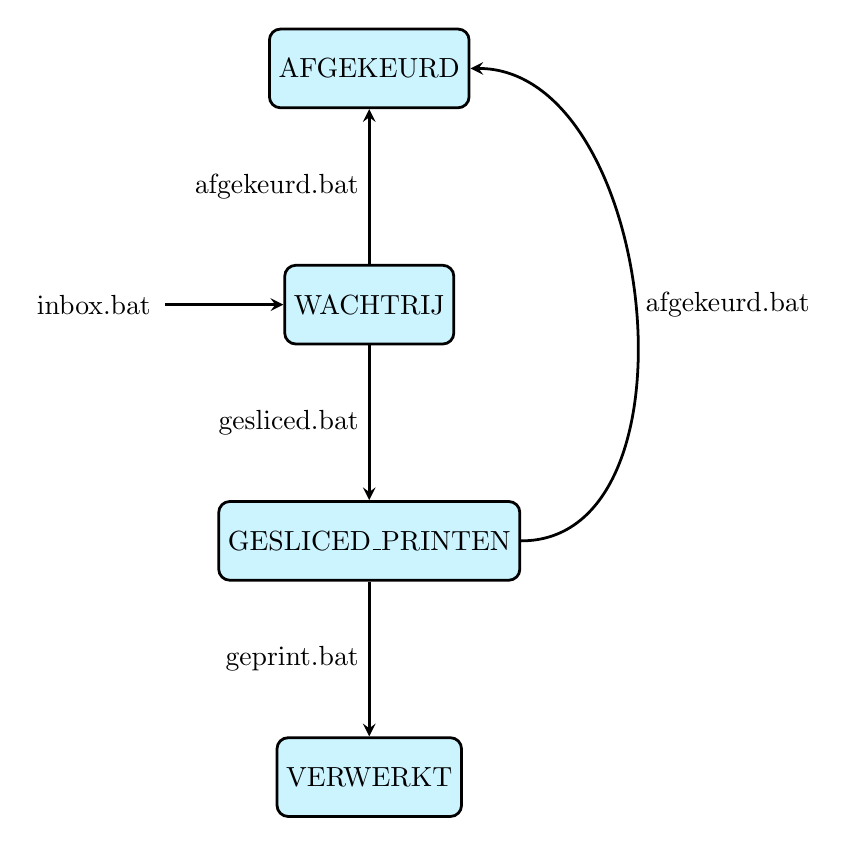
\begin{tikzpicture}[node distance = 3.0cm, line width=1pt]
    % Nodes
    \node [block] (wachtrij) {WACHTRIJ};
    \node [block, above of=wachtrij]  (afgekeurd) {AFGEKEURD};
    \node [block, below of=wachtrij]  (gesliced_printen) {GESLICED\_PRINTEN};
    \node [block, below of=gesliced_printen] (verwerkt) {VERWERKT};

    % arrows
    \draw[>=stealth, ->, line width=1.0pt] ([xshift=-1.5cm]wachtrij.west) to node[xshift=-0.8cm,left]{inbox.bat} (wachtrij.west);
    \draw[>=stealth, ->, line width=1.0pt] (wachtrij.north) to node[left] {afgekeurd.bat} (afgekeurd.south);
    \draw[>=stealth, ->, line width=1.0pt] (wachtrij.south) to node[left] {gesliced.bat} (gesliced_printen.north);
    \draw[>=stealth, ->, line width=1.0pt] (gesliced_printen.east) [out=0, in=0] to node[right] {afgekeurd.bat} (afgekeurd.east);
    \draw[>=stealth, ->, line width=1.0pt] (gesliced_printen.south) to node[left] {geprint.bat} (verwerkt.north);

\end{tikzpicture}
\caption*{Workflow: ingeleverde .stl bestanden worden door .bat functies verplaatst van/naar folders AFGEKEURD, WACHTRIJ, GESLICED\_PRINTEN en VERWERKT}%
\end{figure}

\section*{\hspace{-1cm}Functie Beschrijving:}
\begin{table}[H]
    \centering
    \rowcolors{2}{gray!25}{white}
    \begin{tabular}%
    {>{\raggedright\arraybackslash}p{0.20\textwidth}%
    |>{\raggedright\arraybackslash}p{0.80\textwidth}}
    \rowcolor{myblue}
    Functie & beschrijving\\\hline
    inbox.bat & Vraag of alle \textit{x} binnengekomen mails of een enkele ($x=1$) mail behandeld moet worden. Bij een enkele mail selecteer welke via interactief keuzemenu in de terminal.\newline Maak voor iedere mail die .stl bestanden bevat een folder aan in met naam /Documents/WACHTRIJ/\textit{naam}/ waarbij \textit{naam} de naam is van de persoon die de mail heeft gestuurd. Download de .stl attachments en de binnen gekomen mail naar de respectivelijke \textit{naam} folder. Maak voor ieder van de \textit{x} folders een afkeur.bat functie en plaats deze in de respectivelijke \textit{naam} folder.\\


    afgekeurd.bat & Verplaats de inhoud van de folder waarin afgekeurd.bat zich bevind van de WACHTRIJ of GESLICED\_PRINTEN folder naar de Documents/AFGEKEURD/\textit{MM}-\textit{DD}\_\textit{naam} folder, hierbij is \textit{MM-DD} vandaag. Popup een mail reactie voor met de 'afkeur' handtekening voor de SA om aan te passen en te versturen.\\
    gesliced.bat & Vraag of alle \textit{y} folders in WACHTRIJ of een enkele ($y=1$) folder behandeld moet worden. Bij een enkele folder selecteer welke via interactief keuzemenu in de terminal. Plaats de inhoud van de \textit{y} folders van WACHTRIJ/\textit{naam} in \textit{y} GESLICED\_PRINTEN/\textit{hh}h\_\textit{mm}m\_\textit{naam}/ folders, hierbij is \textit{hh} het aantal uren van de print en \textit{mm} het aantal minuten van de print.
    Maak voor ieder van de \textit{y} folders een geprint.bat functie en plaats deze in de respectivelijke \textit{hh}h\_\textit{mm}m\_\textit{naam} folder.
    \\
    geprint.bat & Verplaats de inhoud van GESLICED\_PRINTEN/\textit{hh}h\_\textit{mm}m\_\textit{naam}/ naar VERWERKT/\textit{MM}-\textit{DD}\_\textit{hh}h\_\textit{mm}m\_\textit{naam}/ waarbij \textit{MM-DD} vandaag is. Popup een mail reactie met de 'geprint' handtekening voor een SA om aan te passen en te versturen.\\
    \end{tabular}
    \caption*{}%
    \label{}
\end{table}


\section*{\hspace{-1cm}Functie Eisen:}
\begin{table}[H]
    \centering
    \rowcolors{2}{gray!25}{white}
    \begin{tabular}%
    {>{\raggedright\arraybackslash}p{0.25\textwidth}%
    |>{\raggedright\arraybackslash}p{0.65\textwidth}}
    \rowcolor{myblue}
    Functie & beschrijving\\\hline
    inbox.bat & thing \\
    afgekeurd.bat & thing \\
    gesliced.bat & thing \\
    geprint.bat & thing \\
    \end{tabular}
    \caption*{}%
    \label{}
\end{table}



\end{document}
